% Template for Elsevier CRC journal article
% version 1.2 dated 09 May 2011

% This file (c) 2009-2011 Elsevier Ltd.  Modifications may be freely made,
% provided the edited file is saved under a different name

% This file contains modifications for Energy Procedia

% Changes since version 1.1
% - added "procedia" option compliant with ecrc.sty version 1.2a
%   (makes the layout approximately the same as the Word CRC template)
% - added example for generating copyright line in abstract

%-----------------------------------------------------------------------------------

%% This template uses the elsarticle.cls document class and the extension package ecrc.sty
%% For full documentation on usage of elsarticle.cls, consult the documentation "elsdoc.pdf"
%% Further resources available at http://www.elsevier.com/latex

%-----------------------------------------------------------------------------------

%%%%%%%%%%%%%%%%%%%%%%%%%%%%%%%%%%%%%%%%%%%%%%%%%%%%%%%%%%%%%%
%%%%%%%%%%%%%%%%%%%%%%%%%%%%%%%%%%%%%%%%%%%%%%%%%%%%%%%%%%%%%%
%%                                                          %%
%% Important note on usage                                  %%
%% -----------------------                                  %%
%% This file should normally be compiled with PDFLaTeX      %%
%% Using standard LaTeX should work but may produce clashes %%
%%                                                          %%
%%%%%%%%%%%%%%%%%%%%%%%%%%%%%%%%%%%%%%%%%%%%%%%%%%%%%%%%%%%%%%
%%%%%%%%%%%%%%%%%%%%%%%%%%%%%%%%%%%%%%%%%%%%%%%%%%%%%%%%%%%%%%

%% The '3p' and 'times' class options of elsarticle are used for Elsevier CRC
%% The 'procedia' option causes ecrc to approximate to the Word template
\documentclass[3p,times,procedia]{elsarticle}

%% The `ecrc' package must be called to make the CRC functionality available
\usepackage{ecrc}

%% The ecrc package defines commands needed for running heads and logos.
%% For running heads, you can set the journal name, the volume, the starting page and the authors

%% set the volume if you know. Otherwise `00'
\volume{00}

%% set the starting page if not 1
\firstpage{1}

%% Give the name of the journal
\journalname{Energy Procedia}

%% Give the author list to appear in the running head
%% Example \runauth{C.V. Radhakrishnan et al.}
\runauth{S. Tarca et al.}

%% The choice of journal logo is determined by the \jid and \jnltitlelogo commands.
%% A user-supplied logo with the name <\jid>logo.pdf will be inserted if present.
%% e.g. if \jid{yspmi} the system will look for a file yspmilogo.pdf
%% Otherwise the content of \jnltitlelogo will be set between horizontal lines as a default logo

%% Give the abbreviation of the Journal.
\jid{egypro}

%% Give a short journal name for the dummy logo (if needed)
\jnltitlelogo{Energy Procedia}

%% Provide the copyright line to appear in the abstract
%% Usage:
%   \CopyrightLine[<text-before-year>]{<year>}{<restt-of-the-copyright-text>}
%   \CopyrightLine[Crown copyright]{2011}{Published by Elsevier Ltd.}
%   \CopyrightLine{2011}{Elsevier Ltd. All rights reserved}
\CopyrightLine{2017}{The Authors. Published by Elsevier Ltd.\\
Peer-review under responsibility of the organising committee of the 1st International Conference on Energy and Power.
}

%% Hereafter the template follows `elsarticle'.
%% For more details see the existing template files elsarticle-template-harv.tex and elsarticle-template-num.tex.

%% Elsevier CRC generally uses a numbered reference style
%% For this, the conventions of elsarticle-template-num.tex should be followed (included below)
%% If using BibTeX, use the style file elsarticle-num.bst

%% End of ecrc-specific commands
%%%%%%%%%%%%%%%%%%%%%%%%%%%%%%%%%%%%%%%%%%%%%%%%%%%%%%%%%%%%%%%%%%%%%%%%%%

%% AMS packages provides various useful mathematical features
\usepackage{amsfonts, amsmath, amssymb, amsthm}
%% Other mathematical packages: arrays, vectors, IEEE equations and mathtools 
\usepackage{array, booktabs, multirow}
\usepackage{esvect}	
\usepackage[retainorgcmds]{IEEEtrantools}
\usepackage{mathtools}
%% Fonts
\usepackage{bbm, dsfont, mathrsfs}		
\usepackage[T1]{fontenc}
%% Footnotes
\usepackage{footmisc}
\usepackage{fnpct}
%% Landscape tables
\usepackage[figuresright]{rotating}
%% URL references
\usepackage{url}


%% The lineno packages adds line numbers. Start line numbering with
%% \begin{linenumbers}, end it with \end{linenumbers}. Or switch it on
%% for the whole article with \linenumbers after \end{frontmatter}.
%% \usepackage{lineno}

%% natbib.sty is loaded by default. However, natbib options can be
%% provided with \biboptions{...} command. Following options are
%% valid:

%%   round  -  round parentheses are used (default)
%%   square -  square brackets are used   [option]
%%   curly  -  curly braces are used      {option}
%%   angle  -  angle brackets are used    <option>
%%   semicolon  -  multiple citations separated by semi-colon
%%   colon  - same as semicolon, an earlier confusion
%%   comma  -  separated by comma
%%   numbers-  selects numerical citations
%%   super  -  numerical citations as superscripts
%%   sort   -  sorts multiple citations according to order in ref. list
%%   sort&compress   -  like sort, but also compresses numerical citations
%%   compress - compresses without sorting
%%
%% \biboptions{comma,round}

% \biboptions{}


%===========================================================================================%
\newcommand{\sqrts}[2][]{\,\sqrt[#1]{#2}\,}

\def\E{\mathbb{E}}
\def\el{l}
\def\given{\,|\,}
\def\I{\mathbb{I}}
\def\N{\mathbb{N}}
\def\one{\mathds{1}}
\def\P{\mathbb{P}}
\def\R{\mathbb{R}}
\def\S{\mathbb{S}}

\def\mwmwh{\delta}
\def\eff{\eta}
%===========================================================================================%
% Hyphenation exception list
\hyphenation{arbi-trage decom-posing energy incre-mental penal-ises}

%===========================================================================================%
% declarations for front matter
\begin{document}

\begin{frontmatter}
\enlargethispage{0pt}
%\newgeometry{top=-2.0cm,bottom=1.0cm}

%% Title, authors and addresses

%% use the tnoteref command within \title for footnotes;
%% use the tnotetext command for the associated footnote;
%% use the fnref command within \author or \address for footnotes;
%% use the fntext command for the associated footnote;
%% use the corref command within \author for corresponding author footnotes;
%% use the cortext command for the associated footnote;
%% use the ead command for the email address,
%% and the form \ead[url] for the home page:
%%
%% \title{Title\tnoteref{label1}}
%% \tnotetext[label1]{}
%% \author{Name\corref{cor1}\fnref{label2}}
%% \ead{email address}
%% \ead[url]{home page}
%% \fntext[label2]{}
%% \cortext[cor1]{}
%% \address{Address\fnref{label3}}
%% \fntext[label3]{}

\dochead{1st International Conference on Energy and Power, ICEP2016, 14--16 December 2016,\\
RMIT University, Melbourne, Australia
}
%% Use \dochead if there is an article header, e.g. \dochead{Short communication}
%% \dochead can also be used to include a conference title, if directed by the editors
%% e.g. \dochead{17th International Conference on Dynamical Processes in Excited States of Solids}

\title{Dispatchability of Wind Power with Battery Energy Storage\\in South Australia}

%% use optional labels to link authors explicitly to addresses:
%% \author[label1,label2]{<author name>}
%% \address[label1]{<address>}
%% \address[label2]{<address>}

\author[acems]{Silvio Tarca\corref{corst}}
\author[acems]{Matthew Roughan}
\author[cet]{Nesimi Ertugrul}
\author[acems]{Nigel Bean}

\address[acems]{School of Mathematical Sciences and ARC Centre of Excellence for Mathematical \& Statistical Frontiers,\\The University of Adelaide, South Australia 5005}
\address[cet]{School of Electrical \& Electronic Engineering and Centre for Energy Technology,\\The University of Adelaide, South Australia 5005}
\cortext[corst]{Corresponding author. \textit{Telephone:} +61 (0)8 8313 4178.  \textit{Email:} \url{silvio.tarca@adelaide.edu.au}}

\begin{abstract}
In fiscal year 2016, 42\% of electricity generated in South Australia came from intermittent renewable energy sources --- a level of penetration that presents challenges to the economic supply of baseload power of acceptable quality.  This study measures the improvement in the dispatchability of intermittent renewable energy from an SA wind farm coupled with a utility-scale battery using model predictive control and real-world data published by the Australian Energy Market Operator.  The process of wind power dispatch with battery energy storage is represented as an incremental state-space model.  The state-space model properly accounts for battery charge/discharge efficiency, and its incremental formulation allows the controller to penalise control effort.
\end{abstract}

\begin{keyword}
%% keywords here, in the form: keyword \sep keyword
Wind power dispatch \sep battery energy storage \sep baseload power \sep time shifting \sep model predictive control \sep state-space model.
%% PACS codes here, in the form: \PACS code \sep code

%% MSC codes here, in the form: \MSC code \sep code
%% or \MSC[2008] code \sep code (2000 is the default)

\end{keyword}

\end{frontmatter}

%%
%% Start line numbering here if you want
%%
% \linenumbers

%===========================================================================================%
% INTRODUCTION																				 %
%===========================================================================================%
\section{Introduction}
The Australian Energy Market Operator (AEMO) reports that of the electricity generated in the state of South Australia (SA) in fiscal year 2016, 35\% and 7\%, respectively, came from wind and solar photovoltaic \cite{SAER16}.  At this level of intermittent renewable energy penetration the challenge is to economically supply baseload power of acceptable quality.  This paper examines the dispatchability of wind power with battery energy storage in SA using state-space model predictive control (MPC).  Improving dispatchability would permit time shifting of wind power dispatched to the electricity grid, enabling wind generators to supply baseload power, exploit energy arbitrage and provide ancillary services.  

The contribution of this research is both theoretical and empirical.  Our theoretical contribution represents the process of wind power dispatch with battery energy storage as an incremental state-space model.  The state-space model properly accounts for battery charge/discharge efficiency, and its incremental formulation allows the MPC controller to penalise control effort.  On an empirical level, we demonstrate the improvement in the dispatchability of intermittent renewable energy by simulating power dispatched to the grid by an SA wind farm coupled with a utility-scale battery at varying levels of confidence.  Using unconstrained intermittent generation forecasts (UIGF) produced by the Australian Wind Energy Forecasting System (AWEFS) and published by AEMO, we find that the probability of power dispatched to the grid supplying a target baseload power is moderately higher with battery energy storage than no energy storage.

A number of recent studies use state-space MPC to demonstrate the improvement in wind power dispatch with battery energy storage.  Their common objective is to minimise the tracking error of actual power dispatched to the grid relative to set points generated using, among other data, wind power forecasts.  They implement MPC controllers that enable wind farms to: schedule power dispatched to the grid \cite{HALBB14,TBBH10}; minimise cost by prolonging battery life \cite{KS10,YCTL12}; maximise revenue by exploiting energy arbitrage \cite{KKSA13}; or supply quality power through the provision of ancillary services \cite{YCTL14}.  The state-space models developed in prior papers are not of the incremental type, and do not penalise control effort.  Nor do they properly account for battery charge/discharge efficiency, instead, either assuming 100\% efficiency or approximating energy losses independent of the power stored or discharged during the dispatch interval.

%===========================================================================================%
% STATE-SPACE MPC OF WIND POWER DISPATCH WITH BATTERY ENERGY STORAGE						 %
%===========================================================================================%
\section{State-Space Model Predictive Control of Wind Power Dispatch with Battery Energy Storage}\label{sect:ssmpc_dispatch}
Our research examines the dispatchability of intermittent renewable energy by simulating power dispatched by an SA wind farm coupled with a utility-scale battery using state-space \textit{model predictive control} (MPC).  A \textit{state-space model} represents a physical process by describing its outputs as a function of state variables, which depend on control signals or process inputs.  The MPC controller determines a sequence of control signals over a given control horizon that results in a sequence of predicted process outputs over a specified prediction horizon, which tracks a sequence of set points or reference signals.  The resulting trajectory of predicted process outputs is an outcome of optimising a \textit{performance index}, or minimising a cost function, that penalises the tracking error of the predicted process outputs relative to their set-point trajectory and the control effort involved in tracking the set-point trajectory.  

%===========================================================================================%
% Incremental State-Space Model																	 %
%===========================================================================================%
\subsection{Incremental State-Space Model}\label{sect:state_space_model}
In the incremental formulation of the state-space model, the control signals become internal state variables augmenting the observable state variables, and control increments serve as process inputs.  We begin by formulating a single-period incremental state-space model in the standard notation typically used to represent an abstract process.  Then, we define the process outputs, state variables and control signals that capture the process dynamics of wind power dispatch with battery energy storage, and formulate the representative incremental state-space model for a single period.

Time in the incremental state-space model is represented as discrete time steps, or intervals, $t\in\N$.  Suppose that discrete times $t\!-\!1$ and $t$, respectively, translate to clock times $\varsigma$ and $\tau$.  Then, ``at time~$t$'' refers to clock time~$\tau$, and ``during time interval~$t$'' refers to clock time interval $(\varsigma, \tau]$.

Let ${\boldsymbol{y}(t)\in\R^{m}}$ be the process output vector at time~$t$, ${\boldsymbol{x}(t)\in\R^{s-q}}$ the observable state vector at time~$t$, and ${\boldsymbol{u}(t)\in\R^{q}}$ the control signal vector at time~$t$.  Denote by ${\boldsymbol{z}(t)\in\R^{s}}$ the augmented state vector at time~$t$, and ${\boldsymbol{\Delta{u}}(t)\in\R^{q}}$ the control increment vector at time~$t$.  Then, the single-period incremental state-space model representing an abstract process may be expressed as 
\begin{IEEEeqnarray*}{rCl}
	% State matrix equation
	\boldsymbol{z}(t\!+\!1) & = &
	\begin{bmatrix*}[c]
		\boldsymbol{x}(t\!+\!1)	\\
		\boldsymbol{u}(t)
	\end{bmatrix*}
	= A
	\begin{bmatrix*}[c]
		\boldsymbol{x}(t)		\\
		\boldsymbol{u}(t\!-\!1)
	\end{bmatrix*}
	+ B\left(\boldsymbol{u}(t) - \boldsymbol{u}(t\!-\!1)\right) = A\boldsymbol{z}(t) + B\boldsymbol{\Delta{u}}(t),\IEEEyesnumber\label{eqn:ssm_state}\\
	% Process output matrix equation
	\boldsymbol{y}(t\!+\!1) & = & C\boldsymbol{z}(t\!+\!1) = CA\boldsymbol{z}(t) + CB\boldsymbol{\Delta{u}}(t),\IEEEyesnumber\label{eqn:ssm_output}
\end{IEEEeqnarray*}
where $A\in\R^{s\times{s}}$, $B\in\R^{s\times{q}}$ and $C\in\R^{m\times{s}}$ are matrices defining the incremental state-space model.

Our incremental state-space model for wind power dispatch with battery energy storage includes two process outputs, four state variables and three control increments.  Let ${e(t) \geq 0}$ be the state of charge (SOC) of the battery at time~$t$, ${p_{b+}(t) \geq 0}$ the battery charge control signal at time~$t$, and ${p_{b-}(t) \geq 0}$ the battery discharge control signal at time~$t$.  We assume that the battery charge control signal diverts wind-generated power to the battery, while the battery discharge control signal dispatches battery power to the electricity grid.  Denote by ${\eff\in(0,1]}$ the one-way charge/discharge efficiency of the battery, and ${\mwmwh > 0}$ the conversion factor from MW to MWh for a given dispatch interval.  Then, the battery SOC is given by
\begin{IEEEeqnarray*}{rCl}
	e(t\!+\!1) & = & e(t) + {\mwmwh\eff}p_{b+}(t) -  \frac{\mwmwh}{\eff}p_{b-}(t)	.	\IEEEyesnumber\label{eqn:bess_soc}
\end{IEEEeqnarray*}

Let ${p_{d}(t) \geq 0}$ be the power dispatched from the wind farm to the grid during time interval~$t$, and ${p_{w}(t) \geq 0}$ the wind power control signal at time~$t$.  In the context of the empirical analysis presented in this paper, $p_{d}(t)$ represents \textit{baseload power}, which we broadly define as the dependable supply of electricity to meet a minimum continuous level of operational demand.  Then, power dispatched to the grid is given by
\begin{IEEEeqnarray*}{rCl}
	p_{d}(t\!+\!1) & = & p_{b-}(t) - p_{b+}(t) + p_{w}(t),\IEEEyesnumber\label{eqn:power_disp_grid}
\end{IEEEeqnarray*}
where ${p_{b}(t) = p_{b-}(t) - p_{b+}(t)}$ is the battery power control signal at time~$t$.  Hence, we follow the convention that $p_{b}(t)$ takes a positive value whenever battery power is discharged and dispatched to the grid, and takes a negative value whenever wind-generated power is diverted from the grid to charge the battery.  Decomposing the battery power control signal into charge and discharge control signals correctly accounts for battery charge/discharge efficiency, as well as accommodating different ranges for charge and discharge rates.  Note that control signals $p_{w}(t)$ and $p_{b}(t)$, and hence $p_{b+}(t)$ and $p_{b-}(t)$, resolved at time~$t$ apply during time interval~$t\!+\!1$.

Accordingly, we define the augmented state, control increment and process output vectors at time~$t$ as
\begin{IEEEeqnarray*}{rCl}
	\boldsymbol{z}(t) & = & \begin{bmatrix*}[c] e(t) & p_{b+}(t\!-\!1) & p_{b-}(t\!-\!1) & p_{w}(t\!-\!1) \end{bmatrix*}^{T},\\
	\boldsymbol{\Delta{u}}(t) & = & \begin{bmatrix*}[c] \Delta{p_{b+}}(t) & \Delta{p_{b-}}(t) & \Delta{p_{w}}(t) \end{bmatrix*}^{T},\;\text{and}\\
	\boldsymbol{y}(t) & = & \begin{bmatrix*}[c] e(t) & p_{d}(t) \end{bmatrix*}^{T},\IEEEyesnumber\label{eqn:ssm_yzdu}
\end{IEEEeqnarray*}
respectively, where control increments $\Delta{p_{b+}}(t)$, $\Delta{p_{b-}}(t)$ and $\Delta{p_{w}}(t) \in \R$.  Notice that battery SOC is modelled as a process output and a state variable.  SOC of the battery reached at the end of the current dispatch (time) interval, a process output, is the SOC at the beginning of the next dispatch interval, a state variable.  
The matrices defining the single-period incremental state-space model are then given by
\begin{equation}\label{eqn:ssm_abc}
	A =
	\begin{bmatrix*}[c]
		1	& \mwmwh\eff	& -\mwmwh/\eff	& 0	\\
		0	& 1			& 0			& 0	\\
		0	& 0			& 1			& 0	\\
		0	& 0			& 0			& 1	\\
    	\end{bmatrix*},\;
	B =
	\begin{bmatrix*}[c]
		\mwmwh\eff	& -\mwmwh/\eff	& 0	\\
		1			& 0			& 0	\\
		0			& 1			& 0	\\
		0			& 0			& 1	\\
	\end{bmatrix*}\;\text{and}\;
	C =
	\begin{bmatrix*}[c]
		1	& 0	& 0	& 0	\\
		0	& -1	& 1	& 1	\\
	\end{bmatrix*}.
\end{equation}
We represent the process of wind power dispatch with battery energy storage by substituting \eqref{eqn:ssm_yzdu} and \eqref{eqn:ssm_abc} into incremental state-space model \eqref{eqn:ssm_state}--\eqref{eqn:ssm_output}.  This substitution yields a single-period (prediction and control horizons) representation of the process.

%===========================================================================================%
% Performance Index																			 %
%===========================================================================================%
\subsection{Performance Index and Process Constraints}\label{sect:perf_index}
Control signals affecting process outputs are determined by optimising a performance index, which penalises tracking error and control effort.  Let $\boldsymbol{r}(t)\in\R^{m}$ be the set-point, or reference signal, vector at time~$t$.  Then, we define the Euclidean norm ($\ell^{2}$-norm) of the predicted process outputs relative to their set points, $\lVert\boldsymbol{r}(t)-\boldsymbol{y}(t)\rVert_{2}$, as the tracking error.  Similarly, the control effort is defined as the norm of the control increments, $\lVert\boldsymbol{\Delta{u}}(t)\rVert_{2}$.  Optimisation of the performance index amounts to minimisation of a quadratic cost function that assigns weights to tracking error and control effort:
\begin{IEEEeqnarray*}{rCl}
    	f & = & \left\lVert\sqrts{\Omega}\left(\boldsymbol{r}(t\!+\!1)-\boldsymbol{y}(t\!+\!1)\right)\right\rVert_{2}^{2} + \lambda\left\lVert\sqrts{\Psi}\boldsymbol{\Delta{u}}(t)\right\rVert_{2}^{2},	\IEEEyesnumber\label{eqn:quad_cost_func}
\end{IEEEeqnarray*}
where $\lambda \geq 0$ is a scalar weighting coefficient, and $\Omega\in\R^{m\times{m}}$ and $\Psi \in\R^{q\times{q}}$ are positive semidefinite diagonal weighting matrices.  Optimisation of the performance index is subject to process constraints, which take the form of upper and lower bounds on observable and internal state variables, with the latter expressed in terms of control increments.  

Substituting for $\boldsymbol{y}(t\!+\!1)$ in \eqref{eqn:quad_cost_func} with \eqref{eqn:ssm_output}, expanding the cost function, dropping the constant terms and imposing process constraints, we write the quadratic program for wind power dispatch with battery energy storage in standard form:
\begin{IEEEeqnarray*}{rCl}
	\underset{\boldsymbol{\Delta{u}}(t)}{\operatorname{argmin}} & \quad & 
		\frac{1}{2}\boldsymbol{\Delta{u}}(t)^{T}\left(B^{T}C^{T}\Omega{CB} + \lambda\Psi\right)\boldsymbol{\Delta{u}}(t) + \big(CA\boldsymbol{z}(t) - \boldsymbol{r}(t\!+\!1)\big)^{T}\Omega{CB}\boldsymbol{\Delta{u}}(t)	\\
    	\operatorname{subject\ to} & & \underline{\boldsymbol{x}} \preceq \boldsymbol{x}(t\!+\!1) \preceq \overline{\boldsymbol{x}},	\\
	& & \underline{\boldsymbol{\Delta{u}}} \preceq \boldsymbol{\Delta{u}}(t) \preceq \overline{\boldsymbol{\Delta{u}}},\qquad\IEEEyesnumber\label{eqn:perf_index_optm}
\end{IEEEeqnarray*}
where the $\preceq$ operator represents the component-wise inequality between vectors.

Battery power control signal $p_{b}(t)$ instructs that the battery either be charged or discharged.  So, if battery charge control signal ${p_{b+}(t)>0}$, then battery discharge control signal ${p_{b-}(t)=0}$; and if ${p_{b-}(t)>0}$, then ${p_{b+}(t)=0}$.  Otherwise, \eqref{eqn:bess_soc} would overstate energy losses due to charge/discharge efficiency and erroneously calculate battery SOC, ${e(t\!+\!1)}$, while \eqref{eqn:power_disp_grid} would miscalculate power dispatched to the grid, ${p_{d}(t\!+\!1)}$.  In order to ensure linear complementarity --- battery charge and discharge control signals cannot both be different from zero at the same time --- we reformulate \eqref{eqn:perf_index_optm} as a mixed integer quadratic program by introducing an auxiliary binary variable and imposing additional constraints.

%===========================================================================================%
% SIMULATION OF WIND POWER DISPATCH WITH BATTERY ENERGY STORAGE							 %
%===========================================================================================%
\section{Simulation of Wind Power Dispatch with Battery Energy Storage}\label{sect:sim_disp_wind_power_bess}
AEMO classifies generators as ``scheduled'', ``semi-scheduled'' or ``non-scheduled'', with wind generators falling into either the semi- or non-scheduled categories.  The NEM dispatch process deducts available capacity for dispatch by non-scheduled generators from the operational demand forecast to arrive at scheduled demand.  Then, given scheduled demand, the NEM dispatch engine uses dispatch offers submitted by scheduled and semi-scheduled generators to determine generator dispatch levels and price through a single-price reverse auction.  While conventional scheduled generators submit dispatch offers with the quantity of electrical power for sale by price band, semi-scheduled wind generators submit only price offers and AEMO determines their wind power output offered for dispatch using AWEFS \cite{AEMO16b}.  Improving the dispatchability of wind power with battery energy storage could lead to a reclassification of wind farms as scheduled generators in the NEM, which would permit time shifting of wind power dispatched to the electricity grid.  It would enable wind generators to supply baseload power to the grid, exploit energy arbitrage, and provide ancillary services to the power system.

\begin{table}[!t]
\begin{minipage}{\textwidth}		% Required to handle footnotes in table
	\centering
	\caption{Specifications of utility-scale, lithium-ion batteries used in simulations of wind power dispatch.  Per-unit base quantities are 100~MW for power and 100~MWh for energy.\vspace*{1.0em}}
	\label{tbl:bess_specs}
	\begin{tabular}{l r r r r}
		\toprule
		& \multicolumn{4}{c}{Lithium-ion Battery} \\
		& \multicolumn{1}{c}{(1)}	& \multicolumn{1}{c}{(2)}	& \multicolumn{1}{c}{(3)}	& \multicolumn{1}{c}{(4)}	\\
		\midrule
		Energy capacity (p.u.)				& 0.250	& 0.500	& 0.750	& 1.000	\\
		Power rating (p.u.)					& 0.125	& 0.250	& 0.375	& 0.500	\\
		Minimum SOC,\footnote{By convention SOC of a battery is expressed as a percentage of its energy capacity, but here we report SOC per-unit.  Minimum SOC of the battery is 12.5\% of its energy capacity.} $\underline{e}$ (p.u.)	& 0.031	& 0.062	& 0.094	& 0.125	\\
		Maximum SOC,\footnote{Maximum SOC of the battery is 87.5\% of its energy capacity.} $\overline{e}$ (p.u.)	& 0.219	& 0.438	& 0.656	& 0.875	\\
		Initial SOC,\footnote{Initial SOC of the battery, $e(0) = (\underline{e}+\overline{e})/2 = 50\%$ of its energy capacity.}	$e(0)$ (p.u.)	& 0.125	& 0.250	& 0.375	& 0.500	\\
		Maximum charge rate,\footnote{Maximum battery charge/discharge rate is 80\% of its rated power.\label{fn:max_chrg_rt}} $\overline{p}_{b+}$ (p.u.)	& 0.100	& 0.200	& 0.300	& 0.400	\\
		Maximum discharge rate,\footref{fn:max_chrg_rt} $\overline{p}_{b-}$ (p.u.)	& 0.100	& 0.200	& 0.300	& 0.400	\\
		One-way charge/discharge efficiency, $\eff$		& 0.920	& 0.920	& 0.920	& 0.920	\\
		\bottomrule
		\end{tabular}
\end{minipage}
\end{table}

In this paper we report power system quantities on a per-unit (p.u.) basis.  The per-unit system expresses quantities in SI units as a ratio relative to base quantities, in our case, 100~MW for power and 100~MWh for energy.  We conduct an empirical analysis of the Snowtown (stage one) wind farm in the mid-north of SA.  It has a registered generation capacity of 1.0~p.u., and a capacity factor of 38\% over the simulation horizon.  We use dispatch UIGF forecasts produced by AWEFS and published by AEMO \cite{AEMO16a}, which estimate the available capacity for wind power dispatch over a 5-minute horizon with a 5-minute resolution at a 5-minute frequency.  AEMO defines \textit{horizon} as how far in advance the forecast is produced, \textit{resolution} as the period over which the forecast is valid, and \textit{frequency} as how often the forecast is produced \cite{AEMO16b}.

While the Snowtown wind farm has not installed an energy storage system, we suppose that energy storage is provided by a lithium-ion battery.  Computations are repeated for four utility-scale batteries of varying energy capacity and power rating.  Their specifications are reported in Table~\ref{tbl:bess_specs}.  These specifications are not taken from existing battery installations, but they are in the bounds of current technology.  Subject to a 75\% discharge cycle, each utility-scale battery coupled to the SA wind farm can supply electricity at its rated power for one and a half hours.

Our empirical analysis implements a na\"ive dispatch strategy over single-period prediction and control horizons.  Subject to constraints on battery SOC and charge/discharge rates, the strategy charges the battery with surplus wind power whenever the available capacity for dispatch exceeds the set point, and discharges the battery to supplement wind power whenever the available capacity for dispatch is less than the set point.  Simulations compute control signals for 105,408 5-minute dispatch intervals from 1 April 2015 to 31 March 2016.  It follows that the conversion factor from MW to MWh for a 5-minute dispatch interval is $\mwmwh = \tfrac{1}{12}$.  

In the state-space model, process outputs $e(t\!+\!1)$ and $p_{d}(t\!+\!1)$ depend on control signals $p_{b+}(t)$, $p_{b-}(t)$ and $p_{w}(t)$.  The wind power control signal, $p_{w}(t)$, is set to the UIGF forecast produced by AWEFS over horizon~$t$ with resolution~$t\!+\!1$.  For each dispatch interval, optimisation of the performance index determines the battery charge control signal, $p_{b+}(t)$, and battery discharge control signal, $p_{b-}(t)$, by minimising the tracking error of power dispatched to the grid, $p_{d}(t\!+\!1)$, relative to a set point that follows the daily load profile of the season, summer or winter.  In these simulations, performance index~\eqref{eqn:quad_cost_func} does not penalise the tracking error of SOC of the battery, $e(t\!+\!1)$, relative to its set point, nor does it penalise control effort, $\boldsymbol{\Delta{u}}(t)$. 

Figure~\ref{fig:disp_wind_bess} illustrates the improvement in wind power dispatch with battery energy storage relative to no energy storage by plotting the probability of power dispatched to the grid equaling or exceeding a set point representing target baseload power.  Note that the ordinates of the curves in Figure~\ref{fig:disp_wind_bess} are plotted against the average of the set points (abscissas) over the simulation horizon, which are calibrated to the daily load profile of the season.  Consider a target baseload range from 0.15~p.u.\ to 0.60~p.u.\ centred on the capacity factor of the Snowtown wind farm (0.38).  Then, the number of 5-minute dispatch intervals over one full year where power dispatched to the grid equals or exceeds the set point is 10--28\% higher with a utility-scale battery than no energy storage.  Clearly, the magnitude of the improvement in dispatchability depends on the size of the battery (energy capacity and power rating).  Notice, too, that the improvement diminishes with increasing battery size.

The empirical observations discussed here are made in the context of the na\"ive, single-period dispatch strategy described above.  The probability of power dispatched to the grid supplying a target baseload power is not very sensitive to the shape of the load profile or battery charge/discharge efficiency due to the positive autocorrelation of wind power over dispatch intervals.  In relation to the latter parameter, lower capital investment in less efficient energy storage technologies would be weighed against revenue foregone from energy losses.  We reiterate that these observations may not hold for more sophisticated, multi-period dispatch strategies, or other measures of dispatchability.

\begin{figure*}[!t]
	\centering
	\scalebox{0.88}{
		% GNUPLOT: LaTeX picture with Postscript
\begingroup
  \makeatletter
  \providecommand\color[2][]{%
    \GenericError{(gnuplot) \space\space\space\@spaces}{%
      Package color not loaded in conjunction with
      terminal option `colourtext'%
    }{See the gnuplot documentation for explanation.%
    }{Either use 'blacktext' in gnuplot or load the package
      color.sty in LaTeX.}%
    \renewcommand\color[2][]{}%
  }%
  \providecommand\includegraphics[2][]{%
    \GenericError{(gnuplot) \space\space\space\@spaces}{%
      Package graphicx or graphics not loaded%
    }{See the gnuplot documentation for explanation.%
    }{The gnuplot epslatex terminal needs graphicx.sty or graphics.sty.}%
    \renewcommand\includegraphics[2][]{}%
  }%
  \providecommand\rotatebox[2]{#2}%
  \@ifundefined{ifGPcolor}{%
    \newif\ifGPcolor
    \GPcolorfalse
  }{}%
  \@ifundefined{ifGPblacktext}{%
    \newif\ifGPblacktext
    \GPblacktexttrue
  }{}%
  % define a \g@addto@macro without @ in the name:
  \let\gplgaddtomacro\g@addto@macro
  % define empty templates for all commands taking text:
  \gdef\gplbacktext{}%
  \gdef\gplfronttext{}%
  \makeatother
  \ifGPblacktext
    % no textcolor at all
    \def\colorrgb#1{}%
    \def\colorgray#1{}%
  \else
    % gray or color?
    \ifGPcolor
      \def\colorrgb#1{\color[rgb]{#1}}%
      \def\colorgray#1{\color[gray]{#1}}%
      \expandafter\def\csname LTw\endcsname{\color{white}}%
      \expandafter\def\csname LTb\endcsname{\color{black}}%
      \expandafter\def\csname LTa\endcsname{\color{black}}%
      \expandafter\def\csname LT0\endcsname{\color[rgb]{1,0,0}}%
      \expandafter\def\csname LT1\endcsname{\color[rgb]{0,1,0}}%
      \expandafter\def\csname LT2\endcsname{\color[rgb]{0,0,1}}%
      \expandafter\def\csname LT3\endcsname{\color[rgb]{1,0,1}}%
      \expandafter\def\csname LT4\endcsname{\color[rgb]{0,1,1}}%
      \expandafter\def\csname LT5\endcsname{\color[rgb]{1,1,0}}%
      \expandafter\def\csname LT6\endcsname{\color[rgb]{0,0,0}}%
      \expandafter\def\csname LT7\endcsname{\color[rgb]{1,0.3,0}}%
      \expandafter\def\csname LT8\endcsname{\color[rgb]{0.5,0.5,0.5}}%
    \else
      % gray
      \def\colorrgb#1{\color{black}}%
      \def\colorgray#1{\color[gray]{#1}}%
      \expandafter\def\csname LTw\endcsname{\color{white}}%
      \expandafter\def\csname LTb\endcsname{\color{black}}%
      \expandafter\def\csname LTa\endcsname{\color{black}}%
      \expandafter\def\csname LT0\endcsname{\color{black}}%
      \expandafter\def\csname LT1\endcsname{\color{black}}%
      \expandafter\def\csname LT2\endcsname{\color{black}}%
      \expandafter\def\csname LT3\endcsname{\color{black}}%
      \expandafter\def\csname LT4\endcsname{\color{black}}%
      \expandafter\def\csname LT5\endcsname{\color{black}}%
      \expandafter\def\csname LT6\endcsname{\color{black}}%
      \expandafter\def\csname LT7\endcsname{\color{black}}%
      \expandafter\def\csname LT8\endcsname{\color{black}}%
    \fi
  \fi
    \setlength{\unitlength}{0.0500bp}%
    \ifx\gptboxheight\undefined%
      \newlength{\gptboxheight}%
      \newlength{\gptboxwidth}%
      \newsavebox{\gptboxtext}%
    \fi%
    \setlength{\fboxrule}{0.5pt}%
    \setlength{\fboxsep}{1pt}%
\begin{picture}(8162.00,5442.00)%
    \gplgaddtomacro\gplbacktext{%
      \csname LTb\endcsname%
      \put(814,704){\makebox(0,0)[r]{\strut{}0}}%
      \put(814,1151){\makebox(0,0)[r]{\strut{}10}}%
      \put(814,1599){\makebox(0,0)[r]{\strut{}20}}%
      \put(814,2046){\makebox(0,0)[r]{\strut{}30}}%
      \put(814,2493){\makebox(0,0)[r]{\strut{}40}}%
      \put(814,2941){\makebox(0,0)[r]{\strut{}50}}%
      \put(814,3388){\makebox(0,0)[r]{\strut{}60}}%
      \put(814,3835){\makebox(0,0)[r]{\strut{}70}}%
      \put(814,4282){\makebox(0,0)[r]{\strut{}80}}%
      \put(814,4730){\makebox(0,0)[r]{\strut{}90}}%
      \put(814,5177){\makebox(0,0)[r]{\strut{}100}}%
      \put(946,484){\makebox(0,0){\strut{}0.00}}%
      \put(1855,484){\makebox(0,0){\strut{}0.10}}%
      \put(2764,484){\makebox(0,0){\strut{}0.20}}%
      \put(3674,484){\makebox(0,0){\strut{}0.30}}%
      \put(4583,484){\makebox(0,0){\strut{}0.40}}%
      \put(5492,484){\makebox(0,0){\strut{}0.50}}%
      \put(6401,484){\makebox(0,0){\strut{}0.60}}%
      \put(7310,484){\makebox(0,0){\strut{}0.70}}%
    }%
    \gplgaddtomacro\gplfronttext{%
      \csname LTb\endcsname%
      \put(176,2940){\rotatebox{-270}{\makebox(0,0){\strut{}$\P\left(\text{power dispatched} \geq \text{set point}\right)$, \%}}}%
      \put(4355,154){\makebox(0,0){\strut{}Average of set points for power dispatched to the grid, p.u.}}%
      \csname LTb\endcsname%
      \put(1894,1936){\makebox(0,0)[l]{\strut{}No energy storage}}%
      \csname LTb\endcsname%
      \put(1894,1716){\makebox(0,0)[l]{\strut{}Battery (1), energy capacity = 0.25 p.u.}}%
      \csname LTb\endcsname%
      \put(1894,1496){\makebox(0,0)[l]{\strut{}Battery (2), 0.50 p.u.}}%
      \csname LTb\endcsname%
      \put(1894,1276){\makebox(0,0)[l]{\strut{}Battery (3), 0.75 p.u.}}%
      \csname LTb\endcsname%
      \put(1894,1056){\makebox(0,0)[l]{\strut{}Battery (4), 1.00 p.u.}}%
      \csname LTb\endcsname%
      \put(4846,4506){\makebox(0,0)[l]{\strut{}Capacity factor = 0.38}}%
      \put(4846,4730){\makebox(0,0)[l]{\strut{}Registered capacity = 1.0 p.u.}}%
    }%
    \gplbacktext
    \put(0,0){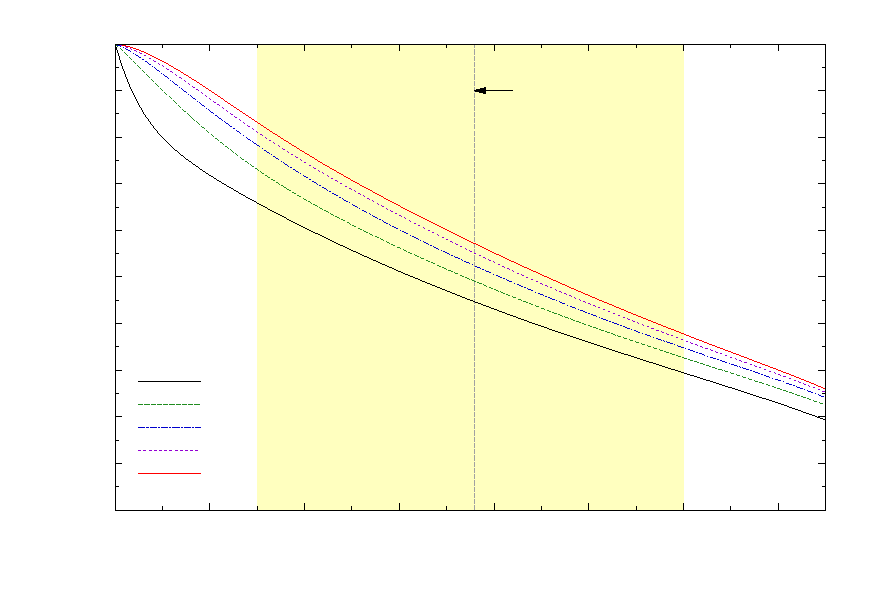
\includegraphics{plot_disp_wind_bess}}%
    \gplfronttext
  \end{picture}%
\endgroup

	}
	\caption[Dispatchability of wind power with battery energy storage]{Probability of power dispatched to the grid equaling or exceeding a set point representing target baseload power.  The set point follows the daily load profile of the season. The MPC controller uses 5-minute dispatch data from 1 April 2015 to 31 March 2016.  Registered generation capacity of the wind farm is 1.0 p.u.  Specifications of the lithium-ion batteries are reported in Table~\ref{tbl:bess_specs}.} 
	\label{fig:disp_wind_bess}
\end{figure*}

This paper does not attempt to make the economic case for installing utility-scale batteries to facilitate time shifting of wind power dispatched to the grid.  But, we remark that as the cost of battery energy storage continues to tumble, utility-scale batteries may become commercially viable in the near- to medium-term.

%===========================================================================================%
% CONCLUSION																				 %
%===========================================================================================%
\section{Conclusion}\label{sect:conclusion}
In this paper we model the process of wind power dispatch with battery energy storage using state-space MPC, and implement a na\"ive, single-period dispatch strategy.  Future research would extend the MPC controller to a multi-period (prediction and control horizons) setting, facilitating the implementation of more sophisticated dispatch strategies.  For example, one that stores surplus intermittent renewable energy during periods of low demand, and discharges the stored energy for dispatch to the grid during periods of high demand when, presumably, prices would be higher.  It would allow wind generators to exploit energy arbitrage.  Moreover, battery energy storage would enable wind generators to participate in ancillary services markets by providing the frequency and voltage regulation that ensures the supply of quality power \cite{ABLFJD12}.

%===========================================================================================%
% ACKNOWLEDGEMENTS																		 %
%===========================================================================================%
%\section*{Acknowledgments}
%Funding for this research is provided by the Australian Research Council through Grant \textit{CE140100049}, and the Australian Renewable Energy Agency through Grant \textit{A00720}.

%===========================================================================================%
% REFERENCES																				 %
%===========================================================================================%
%% Following citation commands can be used in the body text:
%% Usage of \cite is as follows:
%%   \cite{key}         ==>>  [#]
%%   \cite[chap. 2]{key} ==>> [#, chap. 2]
%%

%% References with BibTeX database:

%\bibliographystyle{elsarticle-num}
%\bibliography{sagridnat}

%% Authors are advised to use a BibTeX database file for their reference list.
%% The provided style file elsarticle-num.bst formats references in the required Procedia style

%% For references without a BibTeX database:

\begin{thebibliography}{10}
\expandafter\ifx\csname url\endcsname\relax
  \def\url#1{\texttt{#1}}\fi
\expandafter\ifx\csname urlprefix\endcsname\relax\def\urlprefix{URL }\fi
\expandafter\ifx\csname href\endcsname\relax
  \def\href#1#2{#2} \def\path#1{#1}\fi

\bibitem{SAER16}
{Australian Energy Market Operator}. {S}outh {A}ustralian electricity report.
  \url{http://www.aemo.com.au};
  Aug. 2016.

\bibitem{HALBB14}
Hamalay~D, Antonishen~M, Lajoie~K, Bostrom~A, Brekken~TKA. Improving
  wind farm dispatchability using model predictive control for optimal
  operation of grid-scale energy storage. Energies 2014; 7:5847--5862.

\bibitem{TBBH10}
Teleke~S, Baran~ME, Bhattacharya~S, Huang~AQ. Optimal control of
  battery energy storage for wind farm dispatching. IEEE Transactions on Energy
  Conversion 2010; 25:787--794.

\bibitem{KS10}
Khalid~M, Savkin~AV. A model predictive control approach to the problem of
  wind power smoothing with controlled battery storage. Renewable Energy 2010; 
  35:1520--1526.

\bibitem{YCTL12}
Yao~DL, Choi~SS, Tseng~KJ, Lie~TT. Determination of short-term
  power dispatch schedule for a wind farm incorporated with dual-battery energy
  storage scheme. IEEE Transactions on Sustainable Energy 2012; 3:74--84.

\bibitem{KKSA13}
Khatamianfar~A, Khalid~M, Savkin~AV, Agelidis~VG. Improving wind farm
  dispatch in the {A}ustralian electricity market with battery energy storage
  using model predictive control. IEEE Transactions on Sustainable Energy 2013;
  4:745--755.

\bibitem{YCTL14}
Yao~DL, Choi~SS, Tseng~KJ, Lie~TT. Frequency control ancillary
  service provided by a wind farm: Dual-{BESS} scheme. Journal of Modern Power
  Systems and Clean Energy 2014; 2:93--103.

\bibitem{AEMO16b}
{Australian Energy Market Operator}. Australian wind energy forecasting system.
  \url{http://www.aemo.com.au};
  May 2016.

\bibitem{AEMO16a}
{Australian Energy Market Operator}. Next day dispatch reports.
  \url{http://www.nemweb.com.au}; Apr. 2016.

\bibitem{ABLFJD12}
Aho~J, Buckspan~A, Laks~J, Fleming~P, Jeong~Y, Dunne~F, Churchfield~M,
  Pao~L, Johnson~K. A tutorial of wind turbine control for supporting grid
  frequency through active power control. In: Proceedings of American Control Conference,
  Institute of Electrical and Electronics Engineers. Montr\'eal, Canada; 2012.

\end{thebibliography}

\end{document}

%%
%% End of file `egypro-template.tex'. 